\section{Empirics}

\begin{frame}{实验背景: Fenix International 与乌干达}
  \begin{columns}[T]
    \begin{column}{0.48\textwidth}
      \begin{block}{合作伙伴与 SHS}
        \small
        Fenix International 是乌干达最大的太阳能家庭系统（SHS）供应商。
        \begin{itemize}
          \item 主力产品: 10 瓦系统，可为 LED 灯、收音机、手机充电
          \item PAYGO 模式: 首付 \$5--\$10 $\rightarrow$ 移动支付分期 $\rightarrow$ 逾期锁定 $\rightarrow$ 补缴解锁
          \item 实践中物理回收极少发生: 仅少于 5\% 的违约会走到物理回收
        \end{itemize}
      \end{block}
    \end{column}
    \begin{column}{0.48\textwidth}
      \begin{block}{实验产品: 300{,}000 UGX 学费贷款}
        \small
        \begin{itemize}
          \item 规模约 \$81，占家庭年收入约 6\%，占家庭总借贷约 25\%
          \item 申请时需先缴纳 50{,}000 UGX（约 \$13）保证金
          \item 还款安排: 7 天免息期 + 100 天 $\times$ 每天 3{,}000 UGX
          \item 中位 APR 约 92\%，与乌干达小额贷款利率大致一致
        \end{itemize}
      \end{block}
    \end{column}
  \end{columns}
\end{frame}

\begin{frame}{随机化设计: 四组对照}
  \begin{columns}[T]
    \begin{column}{0.53\textwidth}
      \centering
      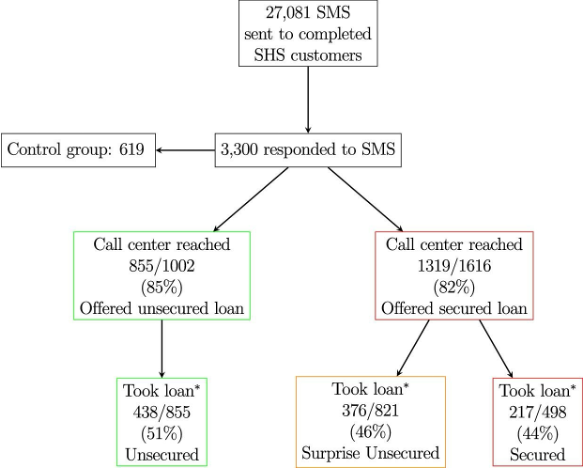
\includegraphics[width=\linewidth,height=0.68\textheight,keepaspectratio]{figures/随机化设计.png}
    \end{column}
    \begin{column}{0.43\textwidth}
      \scriptsize
      \begin{block}{样本起点}
        Fenix 向 27{,}081 名已还清 SHS 贷款的客户发送短信，3{,}300 人（12\%）回复有意向。
      \end{block}

      \begin{block}{四组分配}
        \begin{itemize}
          \setlength{\itemsep}{2pt}
          \item 控制组: 619 人，不主动联系，不提供贷款
          \item 无担保组: 分配 1{,}002 人，成功联系 855 人，最终接受 438 人，接受率 51\%
          \item 惊喜无担保组: 821 人，先被告知需抵押，交保证金后告知其实不用，最终接受 376 人，接受率 46\%
          \item 真正担保组: 498 人，全程都需抵押，最终接受 217 人，接受率 44\%
        \end{itemize}
      \end{block}
    \end{column}
  \end{columns}
\end{frame}

\begin{frame}{识别策略的直觉图示}
  \begin{table}
  \centering
  \scriptsize
  \begin{tabular}{p{3.7cm} p{2.2cm} p{2.5cm} p{2.0cm}}
    \toprule
    \textbf{比较} & \textbf{筛选阶段} & \textbf{还款阶段} & \textbf{识别效应} \\
    \midrule
    Secured vs. Unsecured & $\times$ & $\times$ & \textbf{总效应} \\
    Secured vs. Surprise Unsecured & $\checkmark$（都以为有担保） & $\times$（只有 Secured 被锁定） & \textbf{道德风险} \\
    Surprise Unsecured vs. Unsecured & $\times$（前者正向筛选） & $\checkmark$（都不被锁定） & \textbf{逆向选择} \\
    \bottomrule
  \end{tabular}
\end{table}


  \scriptsize
  惊喜无担保组在\textbf{筛选阶段}模仿 Secured，在\textbf{还款阶段}模仿 Unsecured，因此能把“谁会借”和“借后是否还”拆开。

  \medskip

  \textcite{karlan2009observing} 的分解思路是：
  \begin{itemize}
    \item \textbf{总效应} = Secured vs. Unsecured
    \item \textbf{道德风险} = Secured vs. Surprise Unsecured
    \item \textbf{逆向选择} = Surprise Unsecured vs. Unsecured。
  \end{itemize}
\end{frame}

\begin{frame}{主要结果 I: 筛选、还款与盈利性}
  \begin{table}
  \centering
  \scriptsize
  \begin{tabular}{p{3.1cm} p{2.6cm} p{5.6cm}}
    \toprule
    \textbf{维度} & \textbf{核心数字} & \textbf{解释} \\
    \midrule
    接受率（筛选） & 44\% vs. 51\%，下降约 7 个百分点（$p=0.007$） & 与“数字抵押减少逆向选择”一致: 一部分更可能违约的家庭在事前退出。 \\
    还款率 & 相对无担保贷款的 62\%，提高约 11 个百分点 & 数字抵押显著提高履约率，也提高贷款盈利能力。 \\
    全额偿还率 & 高出约 19 个百分点 & 不仅平均回款增加，右尾的“完全还清”也显著改善。 \\
    机制分解 & 约 $\frac{2}{3}$ 来自道德风险，约 $\frac{1}{3}$ 来自逆向选择 & 惊喜无担保组帮助把“筛选效应”和“激励效应”拆开。 \\
    异质性 & 道德风险主要集中在高风险家庭；逆向选择主要集中在低风险家庭 & 与模型关于不同类型借款人的预测一致。 \\
    \bottomrule
  \end{tabular}
\end{table}


  \scriptsize
  这组结果说明，数字抵押一方面让一部分高违约风险家庭在事前退出，另一方面提高了进入样本家庭在事后的履约激励。结果是贷款人能向更多家庭\textbf{盈利性地}提供信贷。

  \medskip
  \scriptsize 数据与估计结果来自 \cite{gertler2024DigitalCollateral}。
\end{frame}

\begin{frame}{主要结果 II: 教育与资产负债表}
  \begin{table}
  \centering
  \scriptsize
  \begin{tabular}{p{3.1cm} p{2.8cm} p{5.4cm}}
    \toprule
    \textbf{维度} & \textbf{核心数字} & \textbf{解释} \\
    \midrule
    入学率 & 每个孩子入学概率提高约 3 个百分点（88\% $\rightarrow$ 91\%，$p=0.02$） & 对一个有 3 个学龄儿童的中位数家庭，未入学儿童比例约下降 50\%。 \\
    学校相关支出 & 每个孩子增加约 26\%（$p=0.005$） & 学费、校服、学习用品、交通和餐饮支出均上升。 \\
    家庭资产负债表 & 资产购买与出售无显著变化 & 没有证据表明贷款显著恶化家庭资产负债表。 \\
    家庭总借款 & 约增加学费贷款规模的 30\%，但统计上不显著 & 借款扩张的幅度与教育支出增加相当，而非明显推高杠杆。 \\
    \bottomrule
  \end{tabular}
\end{table}


  \scriptsize
  贷款处理显著提高了入学率和学校相关支出，但没有发现家庭资产负债表明显恶化。这说明实验识别出的，不只是“还得更多”，还有真实的人力资本投资改善。
\end{frame}
